% ---------------------------------------------------------------------
% EG author guidelines plus sample file for EG publication using LaTeX2e input
% D.Fellner, v2.02, Jan 25, 2017


\title%
{
%Evaluation of Higher Order Diffusion against Variable Eddington Factor Methods for Rendering Participating Media
$P_N$-Method for Multiple Scattering in Participating Media
}

% for anonymous conference submission please enter your SUBMISSION ID
% instead of the author's name (and leave the affiliation blank) !!
%\author[D. Fellner \& S. Behnke]
%{\parbox{\textwidth}{\centering D.\,W. Fellner\thanks{Chairman Eurographics Publications Board}$^{1,2}$
%        and S. Behnke$^{2}$ 
%        S. Spencer$^2$\thanks{Chairman Siggraph Publications Board}
%        }
%        \\
%% For Computer Graphics Forum: Please use the abbreviation of your first name.
%{\parbox{\textwidth}{\centering $^1$TU Darmstadt \& Fraunhofer IGD, Germany\\
%         $^2$Graz University of Technology, Institute of Computer Graphics and Knowledge Visualization, Austria
%%        $^2$ Another Department to illustrate the use in papers from authors
%%             with different affiliations
%       }
%}
%}

\author[D. Koerner \& J. Portsmouth \& W. Jakob]
{
%Compiled on \today
%paper1027
David Koerner$^{1}$
\qquad Jamie Portsmouth$^{2}$
\qquad Wenzel Jakob$^{3}$
%\qquad Ralf Habel$^{2}$
%\qquad Wojciech Jarosz$^{1,4}$
\\
% For Computer Graphics Forum: Please use the abbreviation of your first name.
$^1$University of Stuttgart
\qquad $^2$Solid Angle
\qquad $^3$\'{E}cole polytechnique f\'{e}d\'{e}rale de Lausanne (EPFL)
%\qquad $^4$Dartmouth College
}


% ------------------------------------------------------------------------

% if the Editors-in-Chief have given you the data, you may uncomment
% the following five lines and insert it here
%
% \volume{36}   % the volume in which the issue will be published;
% \issue{1}     % the issue number of the publication
% \pStartPage{1}      % set starting page


%-------------------------------------------------------------------------
\begin{document}
% uncomment for using teaser
\teaser
{
\centering
\begin{subfigure}{0.24\linewidth}
%\missingfigure{}
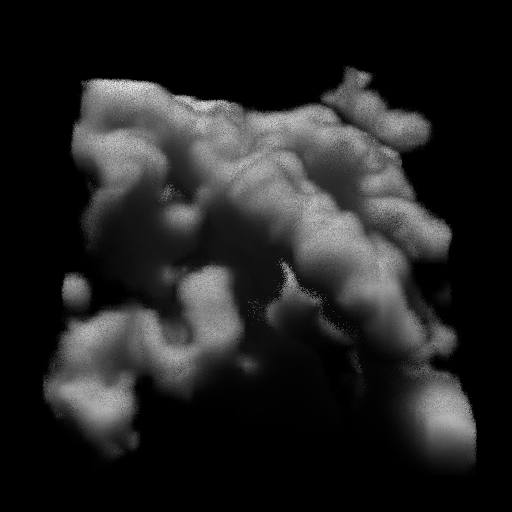
\includegraphics[width=\linewidth]{images/nebulae_ms_cda.png}
\vspace{-0.17in}
\caption{Classical diffusion}
\label{fig:teaser_cda}
\end{subfigure}%
\hspace{0.002\linewidth}
\begin{subfigure}{0.24\linewidth}
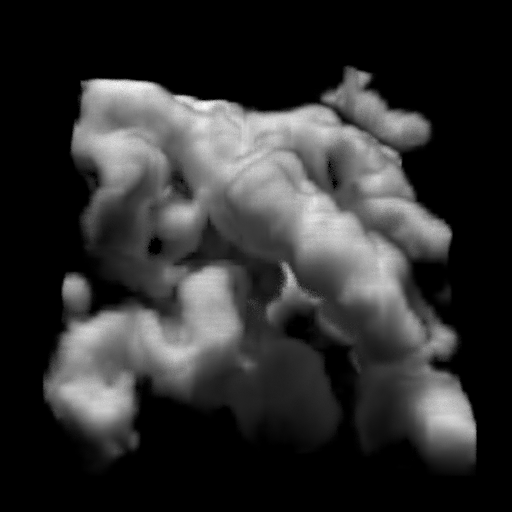
\includegraphics[width=\linewidth]{images/nebulae_ms_p5.png}
\vspace{-0.17in}
\caption{$P_5$ (ours)}
\label{fig:nebulae_ours}
\label{fig:teaser_pn}
\end{subfigure}%
\hspace{0.002\linewidth}
\begin{subfigure}{0.24\linewidth}
%\missingfigure{}
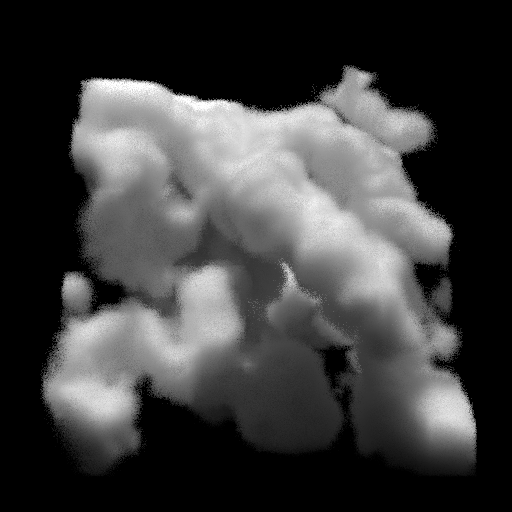
\includegraphics[width=\linewidth]{images/nebulae_ms_fld.png}
\vspace{-0.17in}
\caption{Flux-limited diffusion}
\label{fig:teaser_fld}
\end{subfigure}%
\hspace{0.002\linewidth}
\begin{subfigure}{0.24\linewidth}
%\missingfigure{}
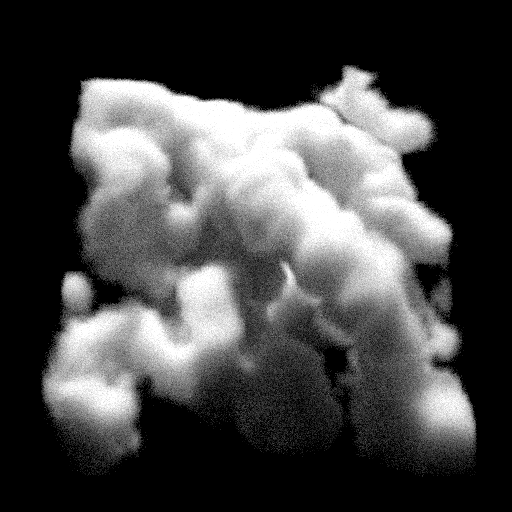
\includegraphics[width=\linewidth]{images/nebulae_ms_groundtruth.png}
\vspace{-0.17in}
\caption{Brute force path tracing}
\label{fig:teaser_gt}
\end{subfigure}%
%\includegraphics[width=\linewidth]{figures/eg_new}
\vspace{-0.1in}
\icaption
{
Flux-limited diffusion (\subref{fig:teaser_fld}) is an extension to the classical diffusion approximation (\subref{fig:teaser_cda}). It improves accuracy, but is based on ad-hoc assumptions about volumetric transport. We add the $P_N$-method (\subref{fig:teaser_pn}) to the toolbox of deterministic methods in rendering and investigate its benefits and tradeoffs against flux-limited diffusion.
}
\label{fig:teaser}
}

\maketitle



%-------------------------------------------------------------------------

\begin{abstract}
%Classical diffusion approximation (CDA) is very competitive for rendering highly scattering participating media, because in these scenarios, Monte Carlo based methods suffer from high computational cost. Variable Eddington Factor methods, such as flux-limited diffusion (FLD), have shown to further improve the results from CDA. In this paper, we look at CDA as a degenerate case of the $P_1$-method and investigate the open question, if going higher order gives a viable alternative to FLD. We derive the time-independent real-valued $P_N$-equations and introduce a framework for generating finite difference stencils directly from the computer algebra representation of the $P_N$-equations for arbitrary order. We further present a staggered-grid $P_N$-solver and compare it against FLD for various standard problems.
Rendering highly scattering participating media using brute force path tracing is a challenge. The diffusion approximation reduces the problem to solving a simple linear partial differential equation. Flux-limited diffusion introduces nonlinearities to alleviate the approximation error but introduces several ad-hoc assumptions. Both methods are based on the spherical harmonics expansion of the radiance field, that is truncated after the first order. In this paper, we investigate the open question of whether higher orders provide a viable alternative to these two approaches. Increasing the order introduces a set of increasingly complex coupled partial differential equations, whose growing number and complexity make them very difficult to work with. We \rev{use} a computer algebra framework for representing and manipulating the underlying mathematical equations and use it to derive the time-independent real-valued $P_N$-equations for arbitrary orders. We further present a staggered-grid $P_N$-solver and generate its stencil code directly from the expression tree of the $P_N$-equations. Finally, we discuss how our method compares to prior work for various standard problems. We will release our computer algebra system, solver, and data as open source to ensure reproducibility of all of our results.
%\begin{classification} % according to http://www.acm.org/class/1998/
%\CCScat{Computer Graphics}{I.3.7}{Three-Dimensional Graphics and Realism}{Raytracing}
%\end{classification}
\end{abstract}



%-------------------------------------------------------------------------
\section{Introduction}

Simulating light transport in paticipating media is still a challenging problem for image synthesis in computer graphics. Monte Carlo based techniques have established as the standard approach, because they can produce unbiased results and are conceptionally easy to implement. They become computationally demanding however, for participating media, which exhibits strong scattering or anisotropy.

Deterministic methods on the other hand are unpopular. This is because they suffer from discretization artifacts, produce biased results, cannot be coupled easily with surface rendering problems and are trickier to implement. However, their appeal lies in the fact that they have better performance for certain problems and produce a global solution across the whole domain.

The work on path guiding techniques from recent years has shown, how discretized approximate representations of the correct solution can be used to accelerate Monte Carlo integration techniques, such as path tracing. Instead of generating these approximate representations using correct methods, deterministic methods may offer a viable alternative and pave the way for hybrid methods, which combine the performance benefits of deterministic methods with correct and exact Monte Carlo techniques. Further, deterministic methods lend themselfs to applications, where a fast approximate solution is often preferred over correct, but slowly converging results. Under this light, it is important to study deterministic methods and have a solid understanding about their characteristics and performance traits for typical rendering problems.

The $P_N$-method is a deterministic method, which is popular in other fields like medical imaging and nuclear sciences, but has not been explored for applications in graphics yet. The purpose and main contribution of our paper is, to gain a solid understanding of its foundations and present a method for application in rendering. In particular, we present the following theoretical and practical contributions:
\begin{itemize}
	\item We derive and present the time-independent real-valued $P_N$-equations.
	\item We introduce a staggered-grid solver, for which we generate stencil code automatically from a computer algebra representation of the $P_N$-equations. This allows us to deal with the increasingly complex equations, which the $P_N$-method produces for higher order. It further allows our solver to be used for any (potentially coupled) partial differential equation, which results in a system of linear equations after discretization.
	\item Finally, we compare the $P_N$-method for higher orders against flux-limited diffusion, and answer the long standing question about which approach should be preferred.
\end{itemize}

In the next section, we will discuss related work and why it motivates our contribution. Section~\ref{sec:pnequations} introduces the real-valued $P_N$-equations, which we solve using our solver described in section~\ref{sec:pnsolver}. We explain in section~\ref{sec:rendering}, how the solution is being applied in a rendering application. Our $P_N$-solver is run and compared against flux-limited diffusion for a set of standard problems in section~\ref{sec:results}. We finish with our conclusion in section~\ref{sec:conclusion}.

%-------------------------------------------------------------------------

\section{Previous work}

Light transport in participating media is governed by the radiative transfer equation~(RTE), first studied in the context of astrophysics by Chandrashekar~\cite{Chandrasekhar60} and later introduced to computer graphics by Kajiya~\cite{Kajiya86}. Today, this equation is typically solved using Monte Carlo methods. In strongly scattering media or in the presence of highly anisotropic phase functions, these methods can become prohibitively expensive. Consider a high albedo media like milk, where tracing paths with many scattering events is necessary.

In contrast to path-tracing, the $P_N$-method gives a solution by solving a system of linear equations. It is derived by discretizing the angular variable of the radiative transfer equation into spherical harmonics (SH). This gives rise to a set of coupled, complex-valued partial differential equations, called $P_N$-equations. The subscript $N$ refers to the truncation order of the spherical harmonics.

The $P_N$-method has a long history in other fields and was never applied in graphics. Kajia~\cite{Kajiya84} explained the theory, but did not give any details on implementation or how to solve it. In fact, as Max~\cite{Max95} pointed out, it is not clear if Kajiya succeeded at all at applying the method, as all of the results in his paper were produced with a simpler method. This is further strengthened by our observation, that a straight forward finite difference discretization of the $P_N$-equations produces unuseable results, due to oscillation artifacts in the solution. In our paper, we derive the real-valued $P_N$-equations along with a staggered-grid solver, that produces artifact free solutions.

\begin{figure}[h]
\centering
\begin{subfigure}{0.45\columnwidth}
%\missingfigure{test}
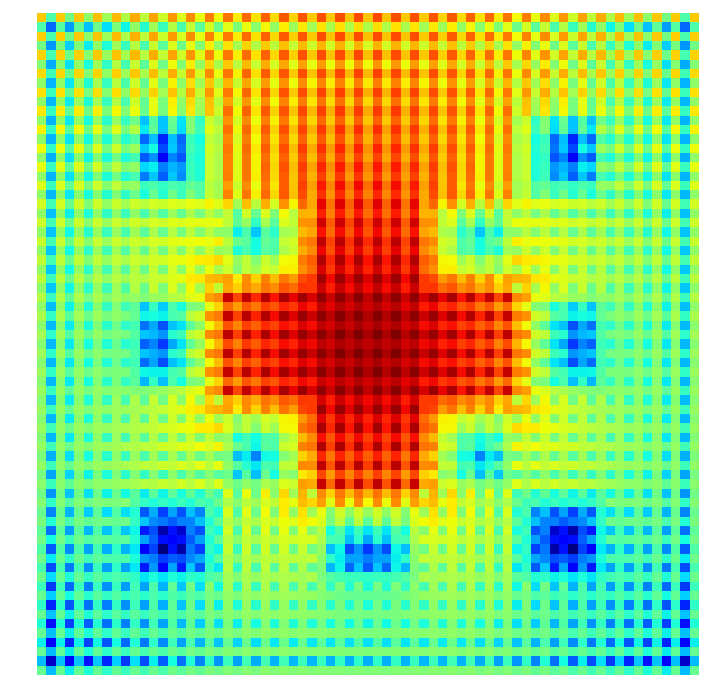
\includegraphics[width=\columnwidth]{images/checkerboard2d_p1_collocated.png}
\end{subfigure}%
\hspace{0.05\columnwidth}
\begin{subfigure}{0.45\columnwidth}
%\missingfigure{test2}
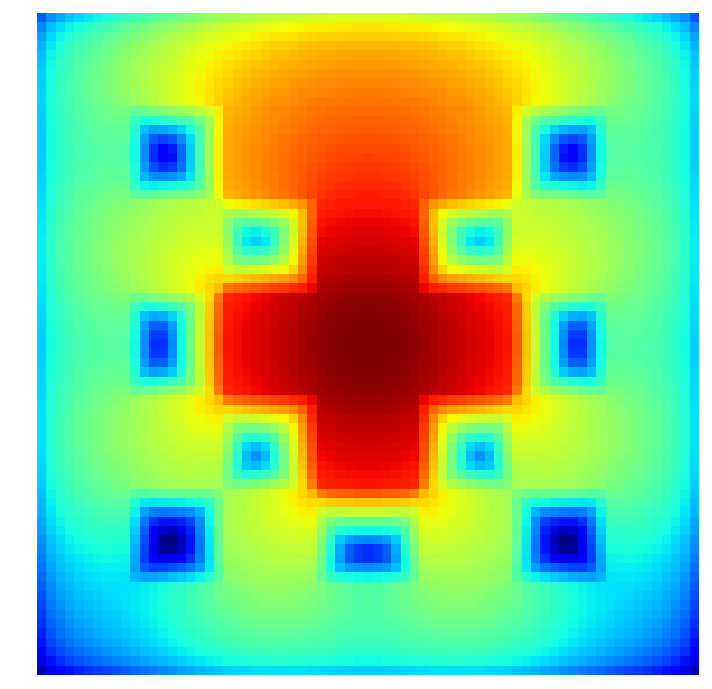
\includegraphics[width=\columnwidth]{images/checkerboard2d_p1_staggered.png}
\end{subfigure}%
\vspace{-0.1in}
\icaption{Solving the 2D checkerboard problem using naive collocated grids produces oscillating artifacts (left). Our solver uses staggered grids and produces artifact free results (right).}
\label{fig:artifacts}
\end{figure}


Similar to $P_N$, the classical diffusion approximation (CDA) is a deterministic method, which arrives at a solution by solving a system of linear equations. It corresponds to the $P_N$-equations when $N=1$ (truncation after the first SH order), which can be collapsed to a simple diffusion equation, giving the method its name. CDA has a long history in other domains, such as astrophysics~\cite{Ishimaru78} and was introduced to graphics by Stam \cite{Stam95}.

CDA suffers from severe energy loss close to regions with strong density gradients. The problem can be addressed by a modification known as Variable Eddington factor (VEF), which nonlinearly adjusts the diffusion coefficient to improve the solution near density gradients and low-density regions. Flux-limited diffusion, developed in the context of astrophysics by Levermore et al.~\cite{Levermore81} and later introduced to graphics by Koerner et al.~\cite{Koerner14}, is the most prominent example.

VEF is based on the observation, that the behavior of volumetric transport is closely linked to the density of the material: In the diffusive regime, thick highly scattering media is present and causes photons to change directions in short succession, while the transport regime in thin and highly absorbing media causes photons to travel long straight lines. In the absence of scattering (e.g. pure vacuum), the non-linear diffusion coefficient turns the diffusion equation into an advection equation. The idea behind VEF is to derive a better diffusion coefficient by seeing it as a mean to spatially blend between the diffusive and pure transport regime.

It is an open and unresolved question, whether the $P_N$-method with truncation at higher order, gives any benefit over using first order non-linear diffusion. This question is also been raised in other domains~\cite{Olson00} and resolving it is one of our motivations.

\vspace{1in}

%\begin{itemize}
  %\item Alternative deterministic methods
  %\begin{itemize}
  %  \item Heuristics \cite{Kaplanyan10} \cite{Elek14}
  %  \item Lattice Boltzmann Methods \cite{Geist04}
  %  \item Discrete Ordinates \cite{Languenou95}
  %\end{itemize}
  %However, among all the deterministic methods, the diffusion approximation has been the most popular due to its intuition and simplicity.


%\end{itemize}



%-------------------------------------------------------------------------
\section{Discretized Radiative Transfer Equation}
\label{sec:discretized_rte}

Our method derives from the radiative transfer equation (RTE), which expresses the change of the radiance field $L$, with respect to an infinitesimal change of position into direction $\omega$ at point $\vec{x}$:
\begin{align}
%\label{eq:rte}
\left(\nabla\cdot\omega\right)L\left(\vec{x}, \omega \right)
=&
-\sigma_t\left(\vec{x}\right) L\left(\vec{x}, \omega \right)\nonumber\\
&
+\sigma_s\left(\vec{x}\right) \int_{\Omega}
{
p\left(\omega'\cdot\omega\right)L\left(\vec{x}, \omega \right)\ud\omega'
}\nonumber\\
&
+Q\left(\vec{x}, \omega\right)\nonumber
\label{eq:rte}
\end{align}

The left hand side (LHS) is the transport term, and we refer to the terms on the right hand side (RHS) as collision, scattering, and source term, respectively. The symbols $\sigma_t$, $\sigma_s$, $p$, and $Q$ refer to the extinction coefficient, scattering coefficient, phase function and emission term.

The RTE is often given in operator notation, where transport, collision, and scattering are expressed as operators $\mathcal{T}$, $\mathcal{C}$ and $\mathcal{S}$, which are applied to the radiance field $L$:
\begin{align}
\mathcal{T}\left(L\right) = -\mathcal{C}\left(L\right) + \mathcal{S}\left(L\right) + Q
\end{align}

Deterministic methods, like ours, are derived by discretizing the angular and spatial domain. This gives rise to a linear system of equations, which can be solved using standard methods. For the $P_N$-method, the angular variable is first discretized, using a truncated spherical harmonics expansion. This results in the $P_N$-equations, a system of coupled PDE's that still depend on a continuous spatial variable.

The number of equations grows with the truncation order $N$. This is why the discretization is hard and error prone if done by hand. We therefore use a computer algebra representation to automate this process. After giving an outline of the general discretization in this section, we will present our computer algebra representation in the next section. The $P_N$-equations that result from our automated discretization are given in Section~\ref{sec:real_valued_pn_eq}. 

Since the radiance field $L$ is real, we use the real-valued SH basis functions $\SHBR^{l,m}$, which are defined in terms of the complex-valued SH basis functions $\SHBC^{l,m}$:
\begin{align}
\SHBR^{l,m}=
\left\{
\begin{array}{lr}
\frac{\iu}{\sqrt{2}}\left(\SHBC^{l,m}-\left(-1\right)^m\SHBC^{l,-m}\right), & \text{for } m < 0\\
\SHBC^{l,m}, & \text{for } m = 0\\
\frac{1}{\sqrt{2}}\left(\SHBC^{l,-m}-\left(-1\right)^m\SHBC^{l,m}\right), & \text{for } m > 0
\end{array}
\right.
\label{eq:sh_real_basis}
\end{align}

We express the projection into the spherical harmonics basis functions with a projection operator $\mathcal{P}$:
\begin{align}
\mathcal{P}^{l, m}(f) = \int_{\Omega}f(\mathbf{x}, \omega) \SHBR^{l,m}(\omega)\,\mathrm{d}\omega = f^{l,m}
\nonumber
\end{align}

The $P_N$-equations are derived by first expressing all direction-dependent parameters in spherical harmonics. The radiance field $L$ in Equation~\ref{eq:rte} is therefore replaced by its SH reconstruction $\widehat{L}$, introducing an error due to truncation at order $N$:
\begin{align}
\widehat{L}\left(\vec{x}, \omega\right) =
\sum_{l=0}^{N}
{
\sum_{m=-l}^{l}
{
L^{l,m}\left(\vec{x}\right)\SHBR^{l,m}\left(\omega\right)
}
}
\approx
L\left(\vec{x}, \omega\right)
\nonumber
\end{align}

After substitution, all angular parameters are expressed in terms of spherical harmonics, but they still depend on the continuous angular variable $\omega$. As a next step, we project each term of the RTE into spherical harmonics, using the projection operator $\mathcal{P}$. This produces a single equation for each $l,m$-pair. The $P_N$-equations therefore can be written as:
\begin{align}
\mathcal{P}^{l,m}\mathcal{T}\left(\widehat{L}\right)
=
-\mathcal{P}^{l,m}\mathcal{C}\left(\widehat{L}\right) 
+\mathcal{P}^{l,m}\mathcal{S}\left(\widehat{L}\right)
+\mathcal{P}^{l,m}\left(Q\right)
\label{eq:pn_operator_notation}
\end{align}

Once the $P_N$-equation have been found, the spatial variable $\vec{x}$ is discretized using a finite difference (FD) voxel grid (using central differences for differential operators).

Following this discretization, the radiance field $L$, is represented as a set of SH coefficients per voxel. Flattening these over all voxels into a single vector, gives the solution vector $\vec{u}$. The RHS vector $\vec{Q}$ is produced similarly. The projected operators can be expressed as linear transformations, which can be collapsed into a single coefficient matrix $A$ (see figure~\ref{fig:matrix_layout}):
\begin{align}
(T+C-S)\vec{u} = A\vec{u} = \vec{Q}
\end{align}

$T$, $C$, $S$ are matrices, which result from the discretized transport, collision and scattering operators respectively.

\begin{figure}[h]
\centering
%\missingfigure{test}
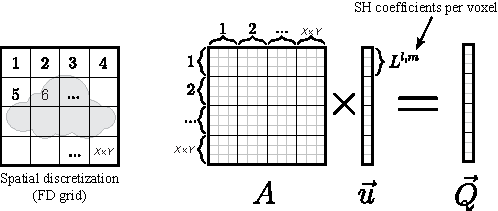
\includegraphics[width=\columnwidth]{figures/fig_matrix_layout.pdf}
\vspace{-0.2in}
\icaption{Structure of coefficient matrix $A$ and solution vector $\vec{u}$ after discretization of the $P_N$-equations on a finite difference grid.}
\label{fig:matrix_layout}
\end{figure}

So far, we have only given the $P_N$-equations in high-level operator notation (Equation~\ref{eq:pn_operator_notation}). Carrying out the full derivation creates large, unwieldy equations and requires a string of expansions, manipulations and applications of identities. These are challenging and error-prone if done by hand. We therefore developed a computer algebra representation, which allowed us to derive the the $P_N$-equation in a semi-automatic fashion.



\section{Computer Algebra Representation}
\label{sec:car}

\rev{We use a computer algebra representation for working with the $P_N$-equations. It represents the equations using a tree of mathematical expressions, which represent numbers, symbols and other expression types, such as integrals, derivatives, sums, products and functions. Further, manipulators can be executed on these expression trees to perform substitution, constant folding, reordering of nested integrals, application of identities and more complex operations. Finally, frontends allow rendering the expression tree into different forms, such as \LaTeX~and C++ source code. While we ended up implementing our own lightweight framework, off-the-shelf packages, such as SymPy (www.sympy.org), exist and would be equally suitable for our use case.}

\begin{figure}[h]
%\vspace{1in}
\centering
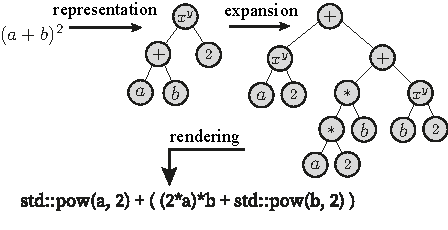
\includegraphics[width=0.9\columnwidth]{figures/fig_car_small.pdf}
%\missingfigure{figures fig car}
\vspace{-0.16in}
\icaption{\rev{A} computer algebra framework allows to represent equations as mathematical expressions trees. It further provides a set of functions for manipulating the tree according to valid mathematical operations, such as the binomial expansion above. Frontends allow generation of source code from the expression tree.}
\label{fig:staggeredgrid}
\end{figure}

\rev{Using the computer algebra representation, we perform the derivation steps required to arrive at the real-valued $P_N$-equations (the derivation steps shown in the supplemental material were almost all rendered from the expression tree). More importantly, we use the representation to perform the discretization and generate the stencil code used by our solver. This is detailed in section~\ref{sec:solver_precomputation}}.






\section{Real-valued $P_N$-Equations}
\label{sec:real_valued_pn_eq}

With the help of \rev{a} computer algebra representation framework, we are able to easily derive and work with the large and unwieldy $P_N$-equations. It is impossible to present the derivation steps in a meaningful way within the scope of this paper. Displaying a single intermediate step could easily take more than ten A4 pages. We therefore decided to give only the final result in this section, and present the derivation in a supplemental document. We present here the final $P_N$-equations, for a general $N$ and in three dimensions, in a very compact form which we have not found elsewhere in the literature

Since the real-valued SH bases (Equation~\ref{eq:sh_real_basis}) have different definitions for $m<0$, $m=0$ or $m>0$,  we also get different projections for $\mathcal{S}^{l,m}$, depending on the sign of $m$.
%\vspace{5in}

%\begin{align}
%&-\frac{1}{2}c^{\scaleto{l-1,m-1}{4pt}}
%\partial_y
%L^{\scaleto{l-1,-m+1}{4pt}}
%%\\
%+\frac{1}{2}d^{\scaleto{l+1,m-1}{4pt}}
%\partial_y
%L^{\scaleto{l+1,-m+1}{4pt}}
%%\\
%-\frac{1}{2}\beta^{\scaleto{m}{4pt}}e^{\scaleto{l-1,m+1}{4pt}}
%\partial_y
%L^{\scaleto{l-1,-m-1}{4pt}}
%\nonumber
%\\&
%+\frac{1}{2}\beta^{\scaleto{m}{4pt}}f^{\scaleto{l+1,m+1}{4pt}}
%\partial_y
%L^{\scaleto{l+1,-m-1}{4pt}}
%%\\
%+\frac{1}{2}\delta_{\scaleto{m\neq -1}{4pt}}c^{\scaleto{l-1,m-1}{4pt}}
%\partial_x
%L^{\scaleto{l-1,m-1}{4pt}}
%\nonumber
%\\&
%-\frac{1}{2}\delta_{\scaleto{m\neq -1}{4pt}}e^{{l-1,m+1}}
%\partial_x
%L^{\scaleto{l-1,m+1}{4pt}}
%%\\
%+\frac{1}{2}f^{\scaleto{l+1,m+1}{4pt}}
%\partial_x
%L^{\scaleto{l+1,m+1}{4pt}}
%%\\
%-\frac{1}{2}d^{\scaleto{l+1,m-1}{4pt}}
%\partial_x
%L^{\scaleto{l+1,m-1}{4pt}}
%\nonumber
%\\&
%+a^{\scaleto{l-1,m}{4pt}}
%\partial_z
%L^{\scaleto{l-1,m}{4pt}}
%%\\
%+b^{\scaleto{l+1,m}{4pt}}
%\partial_z
%L^{\scaleto{l+1,m}{4pt}}
%%\\
%+\sigma_t L^{\scaleto{l,m}{4pt}}
%%\\
%-\sigma_s\lambda_{\scaleto{l}{4pt}}p^{\scaleto{l,0}{4pt}}L^{\scaleto{l,m}{4pt}}
%%\\
%= Q^{\scaleto{l,m}{4pt}}
%\label{eq:rpn_m_<_z}
%\end{align}

For $m=0$ we have
\begin{align}
&
\frac{1}{\sqrt{2}}c^{\scaleto{l-1,-1}{4pt}}\partial_x L^{\scaleto{l-1,1}{4pt}}
-\frac{1}{\sqrt{2}}d^{\scaleto{l+1,-1}{4pt}}\partial_x L^{\scaleto{l+1,1}{4pt}}
%\\&
\frac{1}{\sqrt{2}}c^{\scaleto{l-1,-1}{4pt}}\partial_y L^{\scaleto{l-1,-1}{4pt}}
\nonumber
\\&
-\frac{1}{\sqrt{2}}d^{\scaleto{l+1,-1}{4pt}}\partial_y L^{\scaleto{l+1,-1}{4pt}}
%\\&
+a^{\scaleto{l-1,0}{4pt}}\partial_z L^{\scaleto{l-1,0}{4pt}}
+b^{\scaleto{l+1,0}{4pt}}\partial_z L^{\scaleto{l+1,0}{4pt}}
\nonumber
\\&
+\sigma_t L^{\scaleto{l,m}{4pt}}
-\sigma_s\lambda_{\scaleto{l}{4pt}}p^{\scaleto{l,0}{4pt}}L^{\scaleto{l,m}{4pt}}
= Q^{\scaleto{l,m}{4pt}}\quad ,
\label{eq:rpn_m_=_z}
\end{align}

%and for $m>0$:
%\begin{align}
%&
%\frac{1}{2}c^{\scaleto{l-1,-m-1}{4pt}}\partial_x L^{\scaleto{l-1,m+1}{4pt}}
%%\\&
%-\frac{1}{2}d^{\scaleto{l+1,-m-1}{4pt}}\partial_x L^{\scaleto{l+1,m+1}{4pt}}
%%\\&
%-\frac{1}{2}\beta^{\scaleto{m}{4pt}}e^{\scaleto{l-1,m-1}{4pt}}\partial_x L^{\scaleto{l-1,m-1}{4pt}}
%\nonumber
%\\&
%+\frac{1}{2}\beta^{\scaleto{m}{4pt}}f^{l+1,-m+1}\partial_x L^{\scaleto{l+1,m-1}{4pt}}
%%\\&
%+\frac{1}{2}c^{\scaleto{l-1,-m-1}{4pt}}\partial_y L^{\scaleto{l-1,-m-1}{4pt}}
%\nonumber
%\\&
%-\frac{1}{2}d^{\scaleto{l+1,-m-1}{4pt}}\partial_y L^{\scaleto{l+1,-m-1}{4pt}}
%%\nonumber
%%\\&
%+\delta_{\scaleto{m\neq 1}{4pt}}\frac{1}{2}e^{\scaleto{l-1,-m+1}{4pt}}%\partial_y L^{\scaleto{l-1,-m+1}{4pt}}
%\nonumber
%\\&
%-\delta_{\scaleto{m\neq 1}{4pt}}\frac{1}{2}f^{\scaleto{l+1,-m+1}{4pt}}%\partial_y L^{\scaleto{l+1,-m+1}{4pt}}
%%\\&
%+a^{\scaleto{l-1,-m}{4pt}}\partial_z L^{\scaleto{l-1,m}{4pt}}
%%\nonumber
%%\\&
%+b^{\scaleto{l+1,-m}{4pt}}\partial_z L^{\scaleto{l+1,m}{4pt}}
%\nonumber
%\\&
%+\sigma_t L^{\scaleto{l,m}{4pt}}
%-\sigma_s\lambda_{\scaleto{l}{4pt}}p^{\scaleto{l,0}{4pt}}L^{\scaleto{l,m}{4pt}}
%= Q^{\scaleto{l,m}{4pt}}
%%\nonumber
%\label{eq:rpn_m_>_z}
%\end{align}

and for $m<0$ (upper sign) and $m>0$ (lower sign) we have
\begin{align}
&
\frac{1}{2}c^{\scaleto{l-1,\pm m-1}{4pt}}\partial_x L^{\scaleto{l-1,m\mp 1}{4pt}}
%\\&
-\frac{1}{2}d^{\scaleto{l+1,\pm m-1}{4pt}}\partial_x L^{\scaleto{l+1,m\mp 1}{4pt}}
%\\&
-\frac{1}{2}\beta_x^{\scaleto{m}{4pt}}e^{\scaleto{l-1,m\pm 1}{4pt}}\partial_x L^{\scaleto{l-1,m\pm 1}{4pt}}
\nonumber
\\&
+\frac{1}{2}\beta_x^{\scaleto{m}{4pt}}f^{l+1,\pm m+1}\partial_x L^{\scaleto{l+1,m\pm 1}{4pt}}
%\\&
\mp \frac{1}{2}c^{\scaleto{l-1,\pm m-1}{4pt}}\partial_y L^{\scaleto{l-1,-m\pm 1}{4pt}}
\nonumber
\\&
\pm \frac{1}{2}d^{\scaleto{l+1,\pm m-1}{4pt}}\partial_y L^{\scaleto{l+1,-m \pm 1}{4pt}}
%\nonumber
%\\&
\mp \beta_y^{\scaleto{m}{4pt}}\frac{1}{2}e^{\scaleto{l-1,\pm m+1}{4pt}}\partial_y L^{\scaleto{l-1,-m\mp 1}{4pt}}
\nonumber
\\&
\pm \beta_y^{\scaleto{m}{4pt}}\frac{1}{2}f^{\scaleto{l+1,\pm m+1}{4pt}}\partial_y L^{\scaleto{l+1,-m\mp 1}{4pt}}
%\\&
+a^{\scaleto{l-1,\pm m}{4pt}}\partial_z L^{\scaleto{l-1,\mp m}{4pt}}
%\nonumber
%\\&
+b^{\scaleto{l+1,\pm m}{4pt}}\partial_z L^{\scaleto{l+1,\mp m}{4pt}}
\nonumber
\\&
+\sigma_t L^{\scaleto{l,m}{4pt}}
-\sigma_s\lambda_{\scaleto{l}{4pt}}p^{\scaleto{l,0}{4pt}}L^{\scaleto{l,m}{4pt}}
= Q^{\scaleto{l,m}{4pt}}
\quad ,
%\nonumber
\label{eq:rpn_m_>_z}
\end{align}

with
\begin{align*}
\label{eq:real_sh_basis}
\beta_x^{m}=
\left\{
\begin{array}{ll}
0, & \text{for } m = -1\\
\frac{2}{\sqrt{2}}, & \text{for } m \neq 1\\
1, & \text{otherwise }
\end{array}
\right.
,\quad
\beta_y^{m}=
\left\{
\begin{array}{ll}
\frac{2}{\sqrt{2}}, & \text{for } m = -1\\
0, & \text{for } m \neq 1\\
1, & \text{otherwise }
\end{array}
\right.
\end{align*}

and
\begin{align*}
&
a^{\scaleto{l,m}{4pt}}= \sqrt{\frac{\left(l-m+1\right)\left(l+m+1\right)}{\left(2l+1\right)\left(2l-1\right)}} \qquad
b^{\scaleto{l,m}{4pt}}= \sqrt{\frac{\left(l-m\right)\left(l+m\right)}{\left(2l+1\right)\left(2l-1\right)}}
\\&
c^{\scaleto{l,m}{4pt}}= \sqrt{\frac{\left(l+m+1\right)\left(l+m+2\right)}{\left(2l+3\right)\left(2l+1\right)}} \qquad
d^{\scaleto{l,m}{4pt}}= \sqrt{\frac{\left(l-m\right)\left(l-m-1\right)}{\left(2l+1\right)\left(2l-1\right)}}
\\&
e^{\scaleto{l,m}{4pt}}= \sqrt{\frac{\left(l-m+1\right)\left(l-m+2\right)}{\left(2l+3\right)\left(2l+1\right)}} \qquad
f^{\scaleto{l,m}{4pt}}= \sqrt{\frac{\left(l+m\right)\left(l+m-1\right)}{\left(2l+1\right)\left(2l-1\right)}}
\end{align*}
\begin{align*}
\lambda_l=\sqrt{\frac{4\pi}{2l+1}}
\quad .
\end{align*}

In the next section we will present the solver that we use to solve the $P_N$-equations.
\vspace{1in}

%-------------------------------------------------------------------------
\begin{figure*}[t!]
\centering
%\missingfigure{$P_N$-solver overview: generate stencil code $\rightarrow$ build system $\rightarrow$ solve $\rightarrow$ render}
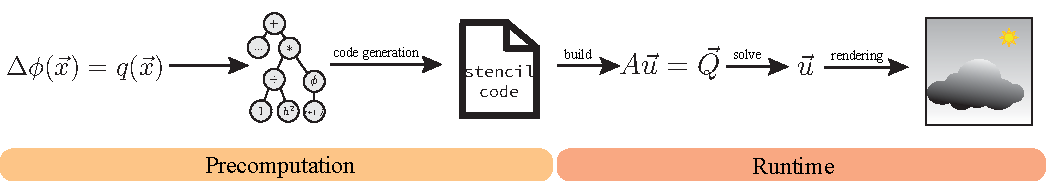
\includegraphics[width=\textwidth]{figures/fig_pipeline.pdf}
\vspace{-0.2in}
\icaption{Overview of our $P_N$-solver. After generating the stencil source code from the expression trees representing the $P_N$-equations, the linear system $A\vec{u}=\vec{Q}$ is built using RTE parameter fields and additional user input, such as grid resolution and type of boundary conditions. The resulting system is solved for $\vec{u}$, which is then used in our rendering application.}
\label{fig:pnsolver}
\end{figure*}

\vspace{-0.75in}

\section{$P_N$-Solver}
\label{sec:pnsolver}

The truncation order $N$ is the key input parameter to the solver. With higher values, manual implementation of the solver from the equations would be arduous, error-prone and time-consuming. We therefore decided to make use of the computer algebra representation and designed our solver around it.

The solver consists of two components. The first is a precomputation (Section~\ref{sec:solver_precomputation}), which is excuted once for every single value of $N$. This steps runs a partial evaluation on the mathematical expression tree and applies the spatial discretization in a reference space we call stencil space. The precomputation step automatically generates source code from the resulting expression tree.

The generated stencil code is compiled with the runtime component (Section~\ref{sec:solver_runtime}) of our solver. This component receives the actual problem as input, including grid resolution and RTE parameter fields. It then builds the linear system and solves it using standard methods. An overview of the solver is given in Figure~\ref{fig:pnsolver}.



\subsection{Precomputation}
\label{sec:solver_precomputation}

The result of the precomputation is a stencil, which can be used during runtime to build the linear system for a given problem. The stencil is a pattern of indices into the solution vector, along with values. It expresses how the sum of the weighted solution vector, components relate to the RHS for a given unknown in the system and therefore contains most information required to fill the system matrix $A$ and RHS-vector $\vec{Q}$ row by row. Note that while the coefficients may change, the sparsity pattern of the stencil is identical for different rows.



\vspace{0.6in}

Stencil generation entails discretizing a PDE at a hypothetical center voxel $(i, j, k)$ (assumed to mean the voxel center most of the time). Finite differences create weighted references to other voxels (e.g. $i+1, j, k$). After bringing the discretized equation into canonical form (a weighted sum of unknowns), one can write the stencil by reading off the weights and offsets (Figure~\ref{fig:stencile_pipeline}). Voxel $(i, j, k)$ will only be known during runtime, when the stencil is executed for a particular unknown (row). Then the offsets can be used to find the component index into the solution-vector, and weights can be evaluated for concrete world space position. We refer to the space with the hypothetical voxel $(i, j, k)$ at the center as stencil space.

\vspace{0.1in}

\begin{figure}[h]
\centering
%\missingfigure{test}
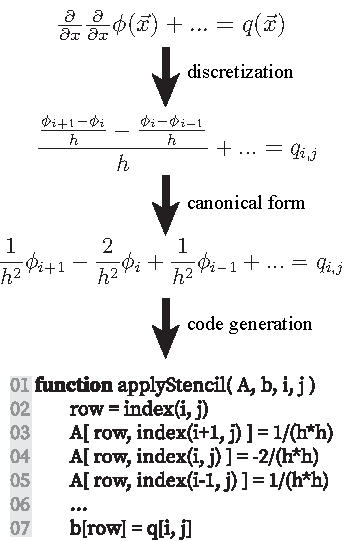
\includegraphics[width=0.7\columnwidth]{figures/fig_stencil_pipeline.pdf}
%\vspace{-0.2in}
\icaption{Creating the stencil code requires several steps, usually done by hand. We express the given problem in a computer algebra representation and use it to fully automate the process.}
\label{fig:stencile_pipeline}
\end{figure}

\vspace{0.2in}

\begin{wrapfigure}{r}{0.6\columnwidth}
%\begin{center}
\hspace{-.2in}
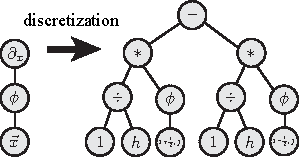
\includegraphics[width=0.6\columnwidth]{figures/fig_discretization.pdf}
%\end{center}
\end{wrapfigure}The spatial discretization is done by parsing the expression tree from the root. The discrete substitute for the continuous position variable $\vec{x}$ is initialized with $ijk$. Differential operator nodes are replaced by a subtree, which expresses the finite difference approximation (including voxelsize factor $h$). The subtree of the differential operator node is duplicated for different offsets to the discrete variable $(i, j, k)$. Since this offset only applies to the subtree, a stack is maintained by the parser to manage scope. Whenever the parser encounters the continuous variable $\vec{x}$ in the expression tree, its node in the tree is replaced by the discrete substitute, currently on top of the stack. Nested differential operators yield higher order finite difference stencils as expected.

\begin{wrapfigure}{r}{0.6\columnwidth}
%\begin{center}
\hspace{-.2in}
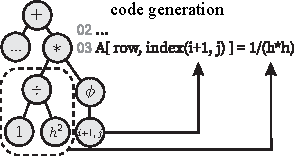
\includegraphics[width=0.6\columnwidth]{figures/fig_codegen.pdf}
%\end{center}
\end{wrapfigure}
Factorization into canonical form is done as a manipulation pass on the mathematical expression tree. The result allows us to implement the code generation in a straightforward fashion. For each term, the $ijk$-offset is retrieved from the unknown. The factor-expression, which is multipled with the unknown, is extracted from the tree and used to generate source code for evaluating the factor-expression during runtime (including calls for evaluating RTE-parameter fields).

\begin{figure}[h]

%\vspace{1in}
\centering
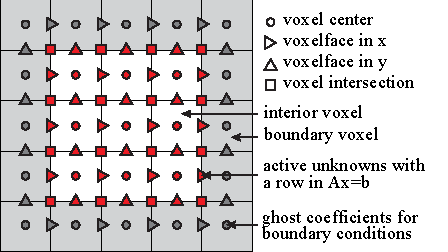
\includegraphics[width=0.9\columnwidth]{figures/fig_staggered_grids.pdf}
%\vspace{-0.2in}
\icaption{Staggered grids place coefficients at different locations within the finite difference grid.}
\label{fig:staggeredgrid}
\end{figure}

\begin{wrapfigure}{r}{0.6\columnwidth}
%\begin{center}
\hspace{-.1in}
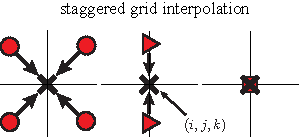
\includegraphics[width=0.6\columnwidth]{figures/fig_staggered_interpolation.pdf}
\vspace{-.1in}
%\end{center}
\end{wrapfigure}Our solver supports placement of coefficients at arbitrary staggered grid locations (see Figure~\ref{fig:staggeredgrid}). This means, that during the discretization step, the discrete location $(i, j, k)$ (at which the unknown is meant to be evaluated) might not coincide with the location of the unknown. To solve this, depending on how the two are located relativeto each other, the parser returns an expression which interpolates the coefficients at $(i, j, k)$ from their defined locations. If those happen to coincide, the coefficient itsself is returned. This is also done for RTE parameters, such as $\sigma_t$ or $p^{l,m}$, which are always located at the voxel center.


%\subsection{Stencil Code Generation}

% After applying the discretization step to the expression tree of the $P_N$-equations, it is used to generate the stencil code. In numerical analysis, a stencil is an arrangement of voxels and weights, that relate values at different locations to each other and form the basis for propagating rows in the system matrix $A$ and RHS vector $\vec{Q}$ with values. The name comes from the fact, that the geometric structure and weights of the configuration do not change, when applied to different voxels. The same is true for the $P_N$-equations and we use this fact to generate a single function, which propagates rows in $A$ and $\vec{Q}$ for a given voxel.

%The $P_N$-equations express, how each coefficient of a voxel depends on other coefficients of the same or adjacent voxels. The unknowns in the terms give information about the coefficient index and voxel offset, and therefore identify a column offset in the matrix $A$. The factors to these coefficients may contain evaluations of RTE parameters, such as $\sigma_t$. Therefore, these factors can not be determined during stencil generation, but are rendered into code expressions, which are executed as part of the stencil function during runtime. Because the stencil code has been generated in stencil space relative to the voxel at $(0,0,0)$, we can run the same stencil code for every voxel, by simply applying an offset accordingly. 



%\subsection{System Building and Solving}
\subsection{Runtime}
\label{sec:solver_runtime}

The stencil code is generated once for every value of $N$ and compiled with the runtime component of our solver. The runtime executes the stencil for every voxel to populate the system matrix $A$ and RHS vector $\vec{Q}$ with numerical values.

The number of rows is determined by the number of voxels times the number of coefficients per voxel (see Figure~\ref{fig:matrix_layout}) and can therefore become very large for high resolution and high truncation order. The matrix $A$ is square and extremely sparse, due to the local structure of the finite differences discretization. Unfortunately, it is non-symmetric due to the transport term and not diagonal dominant, which rules out many \rev{iterative} methods for solving linear systems. \rev{Iterative methods are useful, as they allow balancing accuracy against performance by tweaking the convergence threshold.} We address this by solving the normal form $A^TA\vec{u}=A^T\vec{Q}$ instead. This gives a symmetric and positive definite system matrix $A^TA$, albeit with a higher condition number. Investigation of other solution schemes (e.g. multigrid) would be an interesting avenue for future work. \rev{However, more importantly, in the presence of vacuum regions, the matrix $A$ becomes singular and the system cannot be solved at all. This requires the introduction of a minimum threshold for the extinction coefficient $\sigma_t$.}

Our solver supports Neumann and Dirichlet boundary conditions. They are handled transparently by the code which generates the stencil. Whenever the stencil accumulates coefficients into a boundary location, the framework either ignores the write operation (Dirichlet BC) or accumulates into the row and column in $A$ of the coefficient in the closest voxel inside the domain (Neumann BC). This is done by changing the index of the written component.

%To respect the boundary correctly, additional coefficients (which contribute additional rows and columns in $A$ and $\vec{Q}$) are necessary at boundary voxels. This requires careful managegment and bookkeeping of coefficient indices, which is done transparently by the runtime code.





%\begin{figure}[h]
%\centering
%\begin{subfigure}{0.45\columnwidth}
%%\missingfigure{test}
%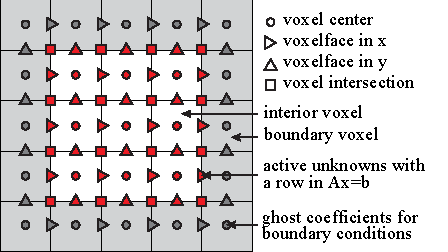
\includegraphics[width=\columnwidth]{figures/fig_staggered_grids.pdf}
%\end{subfigure}%
%\hspace{0.05\columnwidth}
%\begin{subfigure}{0.45\columnwidth}
%\missingfigure{test2}
%\end{subfigure}%
%\vspace{-0.2in}
%\icaption{Staggered grids cause a shifted boundary on the right and upper side of the domain (left). The boundary is correct after introducing additional unknowns (red) at boundary voxels (right).}
%\label{fig:staggeredgrid}
%\end{figure}


%Matrix $A$ and vector $\vec{Q}$ are constructed after applying the stencil for every voxel.



%\subsection*{CDA vs. $P_1$}
%\begin{itemize}
  %\item CDA is a degenerated form of $P_1$. It is derived by isolating the flux-vector on one side of the vector-equation formed by the $l=1$ SH-band equations. This isolation requires division by the extinction coefficient, introducing a $\frac{1}{\sigma_t}$ factor which diverges as $\sigma_t$ approaches zero. Thresholding to some minimum is required, in order to be able to solve the system for vacuum regions.
  %\item $P_1$ does not require any thresholding of $\sigma_t$ as it does not contain $\sigma_t$ as a denominator. It therefore can deal with vacuum regions without modifications.
  %\item (needs validation) Further, in the presence of vacuum or near vacuum regions, the condition number for CDA is higher than for $P_1$, because of small extinction values in the denominator of the diffusion coefficient.
  %\item Using the normal form for CDA will further increase the condition number when vacuum regions are present and significantly decreases convergence.
%\end{itemize}



%-------------------------------------------------------------------------
\section{Rendering}
\label{sec:rendering}

In order to evaluate our results, we chose to use our render the solution directly. We use an approach similar to Koerner et al.~\cite{Koerner14}, where we seperate the radiance field into single scattered light $L_{ss}$ and multiple scattered light $L_{ms}$:
\begin{align}
L\left(\vec{x},\omega\right) = L_{ss}\left(\vec{x},\omega\right) + L_{ms}\left(\vec{x},\omega\right)
\end{align}

The single scattered light is folded into the emission term $Q$:
\begin{align}
Q(\vec{x}, \omega) = L_{ss}(\vec{x}, \omega) = \sigma_s\left(\vec{x}\right)\int_\Omega{ p\left(\omega'\rightarrow\omega\right) L_{u}\left(\vec{x}, \omega'\right)\ud\omega' }
\end{align}

This means that, our solver will solve for the multiple scattered light $L_{ms}$. The quantity $L_u$ is the uncollided light, which was emitted from the lightsource and attenuated by the volume without undergoing any scattering event. It is easily computed for delta light sources, such as directional lights, in homogeneous volumes. Raymarching can be used in heterogeneous volumes. For more complex light sources, the emission field can be precomputed with a number of Monte Carlo iterations. 

Running the solver gives solution vector $\vec{u}$. The staggering is removed by interpolating all coefficients to voxel centers. Also the additional coefficients at boundary voxels are removed. This operation is represented as a matrix and results in a simple three-dimensional voxelgrid with SH coefficients for order $N$ at the center of each voxel.

For rendering, we use a simple forward path tracing approach, where we start tracing from the camera. At the first scattering event, we use next event estimation to account for $L_{ss}$. Then we sample a new direction according to the phase function. Instead of continuing tracing into the new direction, we simply evaluate the inscattering integral using $\widehat{L}_{ms}$. The SH coefficients at $\vec{x}$ are found by trilinear interpolation from the voxelgrid of SH coefficients.




%-------------------------------------------------------------------------
\section{Results}
\label{sec:results}

In this section, we present results for a set of standard problems in order to validate and evaluate our method. We also compare against classical diffusion (CDA) and flux-limited diffusion (FLD).

Our computer algebra framework and the precomputation has been implemented in Python. The runtime component of our solver has been implemented in C++. We use a naive implementation of a CG solver, which has been modified such that we do not need to expliticly compute the normal form of the linear system to solve. We use the sparse matrix representation and sparse matrix vector product from the Eigen linear algebra library.

The solver for classical diffusion is based on the diffusion equation, which is derived by collapsing the $P_1$-equations:
\begin{align} 
\nabla\left(\frac{1}{3\sigma_t}\nabla L^{0,0}\right)  = -Q^{0,0}
\label{eq:cda}
\end{align}

Since our solver can work with any PDE, which results in a linear system of equations, we put Equation~\ref{eq:cda} into our computer algebra representation and provide it as an input to our solver, which would generate the correct stencil code automatically.

Since FLD is based on a non-linear diffusion equation, we were not able to use our system in the same way. Our implementation closely follows the implementation in~\cite{Koerner14} (though ours runs on CPU) and we refer to their paper for more details.

\subsection{2D checkerboard}

First we ran our solver on the 2D checkerboard, a very common test case in other fields. The problem has dimensions $7\times 7$ and is discretized with resolution $71\times 71$. Unit size blocks are filled with purely absorbing medium with $\sigma_a=10$ in a checkerboard pattern. All other blocks are filled with a purely scattering medium with $\sigma_s=1$.

Solving the standard checkerboard problem, allows us to validate our solver against the solver from Seibold et al.~\cite{Seibold14}, which solves for the time-dependent and complex-valued $P_N$-equations in the 2D case only. The 2D case is derived by assuming that all SH coefficients, RTE parameters and boundary conditions are z-independent. This causes all SH coefficients and moment equations for which $l+m$ is odd to vanish. Due to the time-dependency, their approach is to do explicit incremental steps in time. We run their solver for many timesteps, in order to get a result which is close to steady state.

\begin{figure}[h]
\centering
\begin{subfigure}{0.49\columnwidth}
%\missingfigure{test}
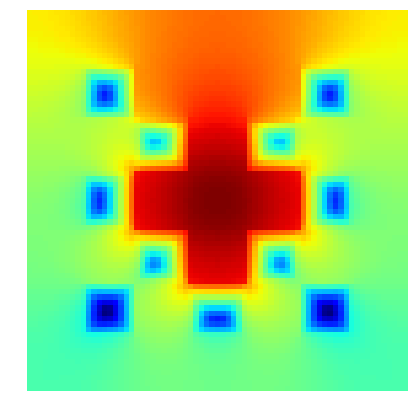
\includegraphics[width=\columnwidth]{images/checkerboard2d_p1_neumann_staggered_starmap.png}
\end{subfigure}%
\hspace{0.01\columnwidth}
\begin{subfigure}{0.49\columnwidth}
%\missingfigure{test2}
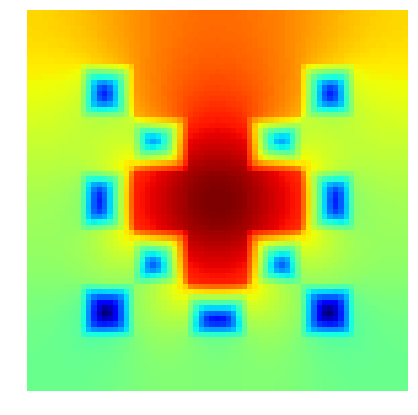
\includegraphics[width=\columnwidth]{images/checkerboard2d_p1_neumann_staggered.png}
\end{subfigure}%
\vspace{-0.2in}
\icaption{Comparison of the result for the checkerboard test using Starmaps time-stepping solver~\cite{Seibold14} (left) against our steady-state solver (right) with $N=5$. Our results are in good agreement.}
\label{fig:vs_starmap}
\end{figure}

As can be seen in figure~\ref{fig:vs_starmap}, the results from our solver are in good agreement with the results from Seibold et al.~\cite{Seibold14} and verify the correctness of our implementation. Converging to a residual of $10e^{-10}$ takes $0.27s$ for $P_1$ and $25s$ for $P_5$.

\subsection{Pointsource problem}

We also run our solver for the point source problem, a single point light in a homogeneous medium. This not only helps to validate our implementation for the 3D case, but also provides information on the accuracy of these methods. We use the Grosjean approximation, which was introduced by D'Eon et al.\cite{dEon11} as a very accurate approximation to the ground truth solution.

\begin{figure}[h]
\centering
\begin{subfigure}{0.45\columnwidth}
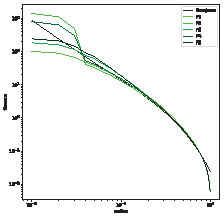
\includegraphics[width=\columnwidth]{figures/pointsource_pn.pdf}
%\missingfigure{test}
\caption{$P_N$ vs. ground truth}
\label{fig:pointsource_pn}
\end{subfigure}%
\hspace{0.05\columnwidth}
\begin{subfigure}{0.45\columnwidth}
%\missingfigure{test2}
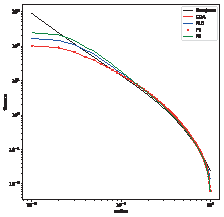
\includegraphics[width=\columnwidth]{figures/pointsource_p5.pdf}
\caption{$P_5$ vs. CDA and FLD}
\label{fig:pointsource_p5}
\end{subfigure}%
\vspace{-0.1in}
\icaption{Lineplot through the 3D solution of our solver for the point source problem for various order $N$ (left). Solution for $P_5$ compared against classical diffusion, flux-limited diffusion and analytical solution (right).}
\label{fig:pointsource}
\end{figure}

For our test case, we choose a FD resolution of $80\times80\times80$, an extinction coefficient $\sigma_t=8.0$ and albedo $\alpha=0.9$. We run the solver for different truncation values $N$. In Figure~\ref{fig:pointsource}~\subref{fig:pointsource_pn}, we see that the solution becomes increasingly accurate for higher truncation order. The ground truth is underestimated when $N$ is odd, and overestimated when $N$ is even. We further see, that the $P_1$ solution exactly matches the results from CDA, which confirmes, that the latter is only a collapsed version of the former. The time to solve is significant with $10m$ for $P_1$ and $45m$ with $P_5$. With these performance characteristics, the $P_N$-method is clearly not competitive in comparison with much diffusion and FLD solver, which are much faster.

\subsection{Nebulae}

Finally, we run our solver on a procedural cloud dataset to get an idea of its performance in more practical applications. Figure~\ref{fig:teaser}~\subref{fig:nebulae_ours} shows the result of $P_5$ for a procedurally generated heterogeneous cloud with an isotropic phase function. We see that at order $N=5$, our method can capture indirect illumination similarily well as FLD and is significantly better than CDA as expected. The indirectly illuminated region at the bottom appears to be closer to the path-traced result as opposed to the solution form FLD which is very flat in that region. However, in many other areas, $P_5$ seems to still suffer a lot from the problem of energy loss near transitions from dense regions to vacuum. It appears that going higher order a few steps, mitigates this problem only slowly at an immense cost of compute and storage.

The main characteristic of the nebulae dataset is the presence of vacuum. We found that having vacuum regions in the dataset will cause the condition number to become infinite and the solver practically doesnt converge. We therefore introduced a minimum threshold for the extinction coefficient $\sigma_t$. Every voxel with an extinction coefficient smaller than the threshold would be set to the threshold value. In Figure~\ref{fig:results_convergence} we show the effect of the minimum threshold on the convergence behavior. As the threshold increases, convergence improves.

%\begin{table}[h]
%\begin{center}
%\begin{tabular}{ c | c c c }
% & \textbf{2D Checkerboard} & \textbf{Point Source} & \textbf{Nebulae} \\ 
%\hline
%$P_1$ & 0.27s & 10m (64\times 64\times 64) & cell6 \\  
%$P_2$ & 2.4s & cell8 & cell9 \\
%$P_3$ & 5.8s & cell8 & cell9 \\
%$P_4$ & 12.7s & cell8 & cell9 \\
%$P_5$ & 25s & ? & ?
%\end{tabular}
%\end{center}
%\icaption{Performance measurements for different datasets and varying truncation order $N$}
%\label{table2}
%\end{table}

\begin{figure}[h]
\centering
%\missingfigure{test}
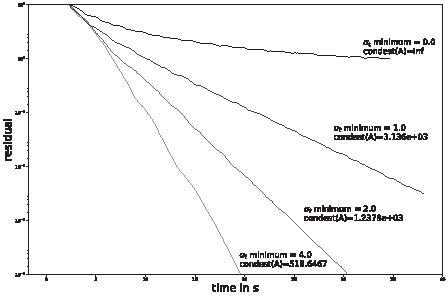
\includegraphics[width=0.9\columnwidth]{figures/fig_nebulae_p1_convergence.pdf}
%\vspace{-0.2in}
\vspace{-0.1in}
\icaption{Convergence behavior of our solver with $N=1$ for the nebulae dataset and for varying minimum thresholds of the extinction coefficient $\sigma_t$. Threshold values and an estimate for the condition number of $A$ (Matlabs condest function) are shown next to the plots. The convergence deteriorates as the threshold decreases. Once it reaches zero, the presence of pure vaccuum makes the condition number infinite.}
\label{fig:results_convergence}
\end{figure}





%\begin{itemize}
%	\item mention performance.
%	\item run for various values of $N$
%	\item convergence behaviour in vacuum. Clearify
%	\item run for anisotropic problem
%\end{itemize}




%-------------------------------------------------------------------------
\section{Conclusion}
\label{sec:conclusion}

In this paper, we introduced the $P_N$-method to the toolbox of deterministic methods for rendering participating media in computer graphics. We derived and presented the real-valued $P_N$-equations, along with a staggered grid solver for solving them. We showed how to use the results in a rendering system and ran our solver for various standard problems for validation.

We originally set out to understand how non-linear diffusion compares to $P_N$ for increasing order. Although the lack of higher moments makes the FLD solution very flat, its energy conserving nature and comparably small resource footprint make it a much better approach when compared to $P_N$, which becomes increasingly costly for higher values of $N$.

\vspace{0.5in}

The literature in other fields often states that the $P_N$ method---when solved in normal form like we do---is able to deal with vacuum regions. We found this misleading. The $P_N$-method in normal form indeed does not break down completely in the presence of vacuum as diffusion based methods do (due to $\sigma_t^{-1}$ in the diffusion coefficient). However, in the presence of vacuum, the condition number of the system matrix becomes infinite and does not converge either. Therefore $P_N$ based methods also require minimum thresholding of the extinction coefficient and offer no benefit for vacuum regions.

Much more work needs to be done in order to make the $P_N$ method competitive in performance to alternative solutions for volume rendering. We believe this can be made possible by employing a multigrid scheme for solving the linear system of equations. We implemented a multigrid solver, but did not find the expected performance improvements. This is possibly due to the coupling between coefficients within a voxel, which does not work well together with the smoothing step. We want to study this in the future.

Unique to our system is that it uses a computer algebra representation of the equation to solve as input. Discretization in angular and spatial domain is done using manipulation passes on the representation. The stencil code, which is used to populate the system of linear equations, is generated from the expression tree. This way, we can easily deal with coupled PDEs and avoid the time consuming and error prone process of writing stencil code by hand.

When researching the application of $P_N$ in other fields, we came across a rich variety of variations on the $P_N$-method, such as simplified $P_N$ ($SP_N$)~\cite{Ryan10}, filtered $P_N$ ($FP_N$)~\cite{Radice13}, diffusion-correction $P_N$ ($DP_N$)~\cite{Schaefer11} and least-squares $P_N$ ($LSP_N$)~\cite{Hansen14}. These variations have been introduced to address certain problems of the standard $P_N$-method, such as ringing artifacts, dealing with vacuum regions and general convergence. Our solver can be applied to any (potentially coupled) PDE and therefore can generate stencil code for all these variations by simply expressing the respective PDEs in our computer algebra representation and providing this as an input to our solver. This would allow an exhaustive comparison of all these methods and we consider this as future work.

Finally, since the approach of our solver is very generic, we also would like to explore its application to other simulation problems in computer graphics.





% --------------------------------------------------------------------------------------------------
\vspace{-0.1in}
\section*{Acknowledgements}
\label{sec:acknowledgements}
\vspace{-0.05in}
We thank the anonymous reviewers for their valuable and encouraging comments and feedback. We also thank Martin Frank and Benjamin Seibold for the very valuable discussions and answers to our questions. We thank Bernd Eberhardt for feedback and support. This project has been partially funded by the MSC-BW project.

%-------------------------------------------------------------------------

\bibliographystyle{eg-alpha}
%\bibliographystyle{eg-alpha-doi}

\bibliography{bibliography}

%-------------------------------------------------------------------------
%\newpage



\end{document}
